\chapter{ヒストグラム}
\label{chap_Histogram}

\section{ヒストグラムとは何か}

ヒストグラム(histogram、度数分布図)は、ある物理量を複数回測定したとき、測定値の分布がどのようになってい るかを表すときに頻繁に使われます。物理学実験で目にする例では、不安定粒子の崩壊時間の分布(指数分布)、結晶シンチレータの発光量の分布(ガウス分布)、光検出器に微弱光を入射したときの検出光電子数の分布(ポアソン分布)などがあります。身近な日常生活の例では、図\ref{fig_population_eps}に示すような人口の年齢分布などに使われます。

\begin{figure}
  \centering
  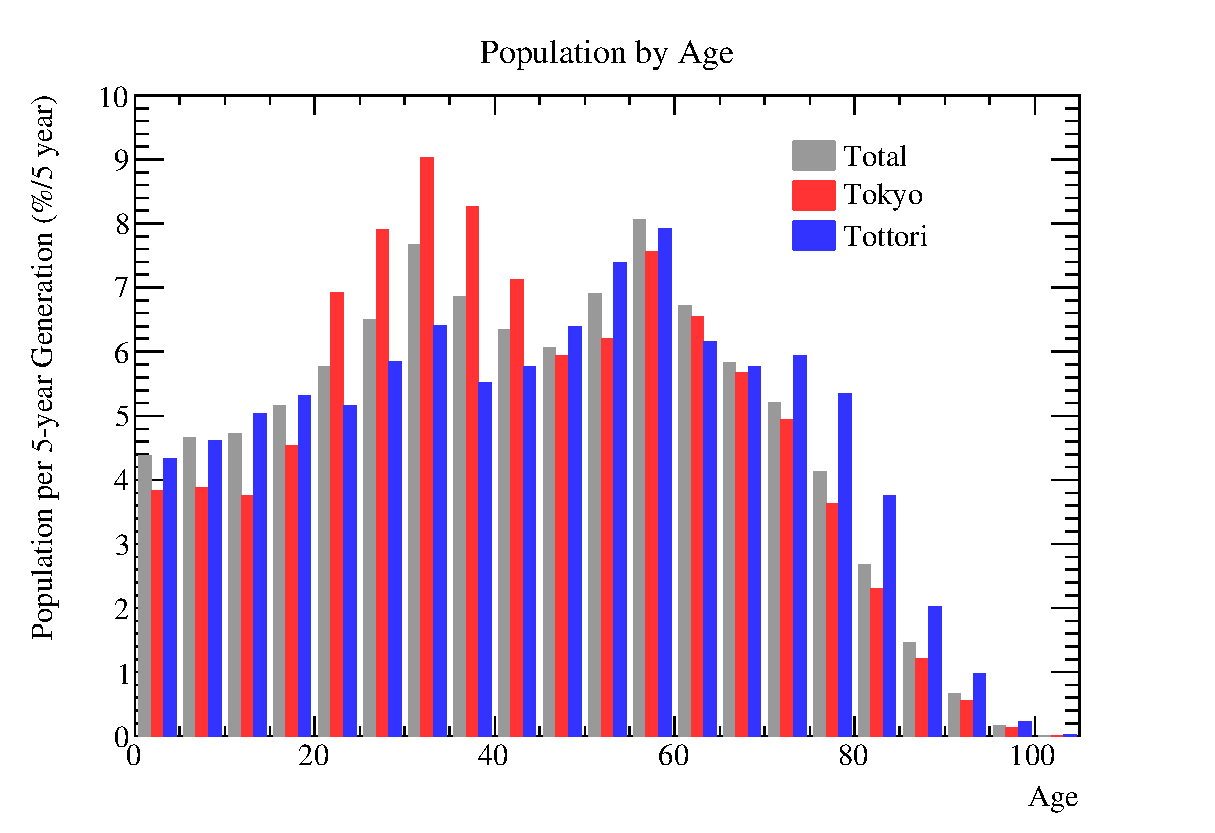
\includegraphics[width=12cm,clip]{fig/population.eps}
  \caption{2005年国勢調査を元にした、全国合計、東京都、島根県の年齢別人口分布。コード\ref{code_frame_fill_color}で同じ結果を得られる。データは\url{http://www.e-stat.go.jp/SG1/estat/List.do?bid=000001007609&cycode=0}から入手可能。}
  \label{fig_population_eps}
\end{figure}

ヒストグラムを使うと、その測定対象がどのような値を取りやすいのかが、一目瞭然になります。図\ref{fig_population_eps}の元データは、総務省統計局のまとめた国勢調査の結果です。コード\ref{code_population_dat}のような、単なる数字の羅列を見ただけでは、このデータがどのような特性を持っているのかを視覚的に認識することは大変困難です。どのような年齢層に人口が偏っているのか、東京のような都市部と鳥取のような地方では、人口分布の特徴がどうなっているのか、こういう情報はヒストグラムにして比較するのが一番です。図\ref{fig_population_eps}と図\ref{fig_population2_eps}は、コード\ref{code_population_C}で作成しました。

%\begin{NoFloat}
\lstinputlisting[language=TeX,float=tb,caption=\texttt{population.dat},label=code_population_dat,numbers=left]{src/population.dat}
%\end{NoFloat}

ヒストグラムを「読む」上で大切な点は、棒の1本ずつの面積が意味を持つということです。図\ref{fig_population_eps}を見ると、0〜5歳の人口は全国平均で約4.5\%になっています。ただし、縦軸の値は「\%」ではなく「\%/5 year」になっていることに注意してください。1つの棒の幅が5年間分あるので、縦軸の値に5年間をかけて、単位が「\%」になった人口の割合が出てくるわけです\footnote{新聞などで見かける図表の多くは、縦軸の単位を省略して単純に「\%」を使うことが多いですが、我々のように物理量を単位を含めて正確に扱う場面では、分母が何であるのか注意してください。}\footnote{図\ref{fig_population_eps}では、3つのヒストグラムを並べて表示するために棒の幅を5年間よりも細くしています。5年間分の太さにするほうがより正確な表現ですが、この図では(本来の幅が常識で判断できるため)見やすさを優先してあります。}。

%\begin{NoFloat}
\lstinputlisting[language=c++,breaklines=true,caption=\texttt{population.C},label=code_population_C,numbers=left]{src/population.C}
%\end{NoFloat}

\subsection{ビン}

図\ref{fig_population_eps}の横軸は、0〜105歳を21の区間に分けてあります。このような小分けした区間のことを、ビン(bin)と呼びます。またそれぞれのビンの幅が5歳分に相当し、これをビン幅(bin width)と呼びます。この例の21という数を、ビン数などと呼ぶことがあります。同じデータに対してビン数を変化させても、ヒストグラムの総面積は一定であることに注意してください。

\subsection{折れ線グラフとの違い}

ヒストグラムの用途は、ある測定値の範囲にどれだけの事象(イベント)が存在するかを図示することです。したがって、測定値には幅が存在し、特定の測定値で代表することはできません。先ほどの図\ref{fig_population_eps}の例では、最初の棒は$0$〜$5$歳の人口を表していました。縦軸の値は、中心値の$2.5$歳を代表するものではないことに注意してください。

従って、図\ref{fig_population_eps}を図\ref{fig_population2_eps}のように折れ線グラフにして表示するのは誤りです。折れ線グラフにする場合は、1つ1つの点の座標がともに(誤差の範囲内で)意味のある1つの数値でなくてはいけません。折れ線グラフを使用するのは、原則として線分の傾きに意味がある場合に限ります。

\begin{figure}
  \centering
  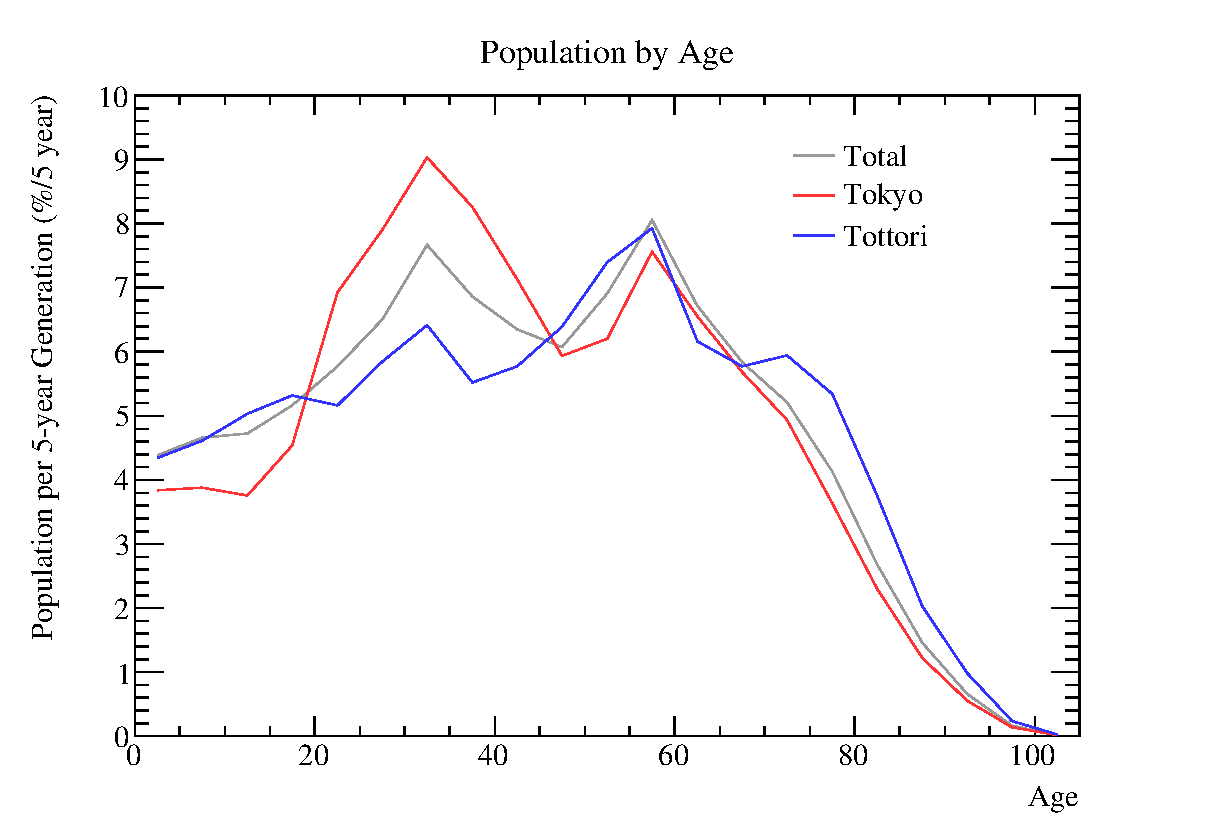
\includegraphics[width=12cm,clip]{fig/population2.eps}
  \caption{図\ref{fig_population_eps}の間違った表示方法の例}
  \label{fig_population2_eps}
\end{figure}

図\ref{fig_population2_eps}では意図的に不適切な表示をしましたが、実際に、研究者といえどもヒストグラムの間違った使い方をしている場合があります。例えば福島第一原発の事故後、東京大学柏キャンパスの柏地区環境安全管理室ではキャンパス内の 空間線量率の測定を行いました\footnote{\url{http://www.kashiwa.u-tokyo.ac.jp/kankyo/ks2011 11/}}。多数の測定点での空間線量率の分布として、図\ref{fig_Kashiwa_png}を掲載しています。

\begin{figure}
  \centering
  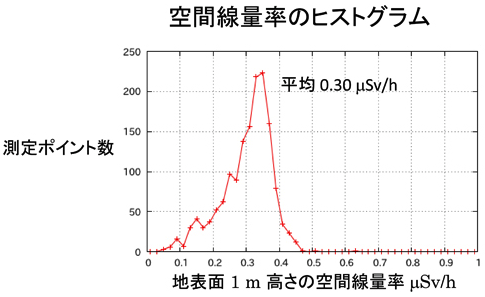
\includegraphics[scale=0.8,bb= 0 0 485 297]{fig/Kashiwa.png}
  \caption{東京大学柏キャンパス内の空間線量率の分布(柏地区環境安全管理室より引用)}
  \label{fig_Kashiwa_png}
\end{figure}

既に説明した通り、図\ref{fig_Kashiwa_png}の表示方法は不適切です。ヒストグラムは棒グラフで描くべきであり、折れ線グラフにし てはいけません。点と点を線で結んで良いのは、その傾きに意味があるときです。図\ref{fig_Kashiwa_png}の縦軸の単位は、正確に書く と「ポイント数/($0.02\ \mu\mathrm{Sv/h}$)」になります\footnote{「ポイント数」は本当は「単位」ではありません。}。しかしヒストグラムが折れ線で結ばれてしまっているため、このグラフ を積分しても、実際の測定点数と同じにはならないでしょう。繰り返しますが、ヒストグラムはどのようなビン幅で作図しても面積は一定です。

\section{1次元ヒストグラム}

それでは、ROOTでどのようにヒストグラムを扱うのか順番に説明します。まずは1次元のヒストグラムからです。 ROOTには1次元のヒストグラムを扱うためのクラスが複数存在します。純粋仮想クラスである\texttt{TH1}、それを継承した\texttt{TH1C}、\texttt{TH1S}、\texttt{TH1I}、\texttt{TH1F}、\texttt{TH1D}です。最初は\texttt{TH1D}だけ覚えておけば十分です\footnote{\texttt{TH1D}は、それぞれのbinに詰まった値が\texttt{Double\_t}型で保存されます。\texttt{TH1C}、\texttt{TH1S}、\texttt{TH1I}、\texttt{TH1F}はbinの値が\texttt{Char\_t}、\texttt{Short\_t}、\texttt{Int\_t}、\texttt{Float\_t}型で保存されます。消費されるメモリの量、整数で値を保持したいかそれとも浮動小数でも良いか、などを考慮して使うヒストグラムのクラスを選択します。}。

それでは\texttt{TH1D}の簡単な使い方の説明です。まずROOTを起動し、次の操作を行って下さい。図\ref{fig_TH1D_eps}のような図が表示されるはずです。

\begin{lstlisting}[language=c++]
root [0] TH1D* hist = new TH1D("hist", "Gaussian Distribution", 100, -10, 10)
root [1] hist->GetXaxis()->SetTitle("Physics Quantity #it{X}")
root [2] hist->GetYaxis()->SetTitle("Entries")
root [3] const Double_t kMean = 3.
root [4] const Double_t kSigma = 2.
root [5] for(Int_t i = 0; i < 10000; i++){
end with ’}’, ’@’:abort > Double_t x = gRandom->Gaus(kMean, kSigma);
end with ’}’, ’@’:abort > hist->Fill(x);
end with ’}’, ’@’:abort > }
root [6] hist->Draw()
Info in <TCanvas::MakeDefCanvas>:  created default TCanvas with name c1
root [7] hist->GetMean()
(const Double_t)3.00946139487923459e+00
root [8] hist->GetMeanError()
(const Double_t)1.98828055273296521e-02
root [9] hist->GetRMS()
(const Double_t)1.98778342044547629e+00
root [10] hist->GetRMSError()
(const Double_t)1.40592666173881657e-02
\end{lstlisting}

\begin{figure}
  \centering
  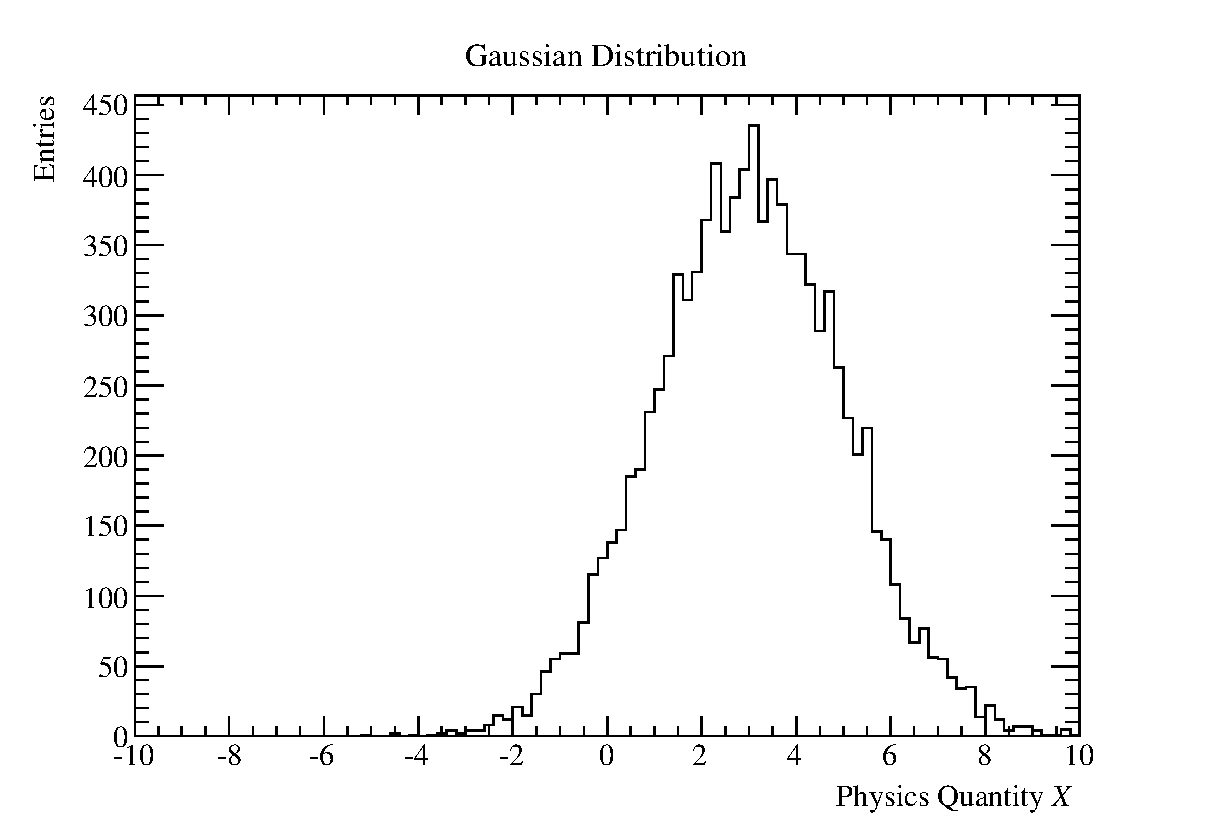
\includegraphics[width=12cm,clip]{fig/TH1D.eps}
  \caption{物理量$X$(平均$\mu = 3$、標準偏差$\sigma = 2$)のガウス分布の例}
  \label{fig_TH1D_eps}
\end{figure}

\section{2次元ヒストグラム}

\begin{lstlisting}[language=c++]
root [0] TH1D* h1 = new TH1D("h1", "1D Gaussian Distribution;#it{r};Entries", 50, 0, 10)
root [1] TH2D* h2 = new TH2D("h2", "2D Gaussian Distribution;#it{x};#it{y};Entries", 100, -10, 10, 100, -10, 10)
root [2] const Double_t kSigma = 2.
root [3] for(Int_t i = 0; i < 100000; i++){
end with ’}’, ’@’:abort > Double_t x = gRandom->Gaus(0, kSigma);
end with ’}’, ’@’:abort > Double_t y = gRandom->Gaus(0, kSigma);
end with ’}’, ’@’:abort > h2->Fill(x, y);
end with ’}’, ’@’:abort > }
root [4] TCanvas* can = new TCanvas("can", "can", 600, 600)
root [5] h2->Draw("colz")
\end{lstlisting}

\begin{figure}
  \centering
  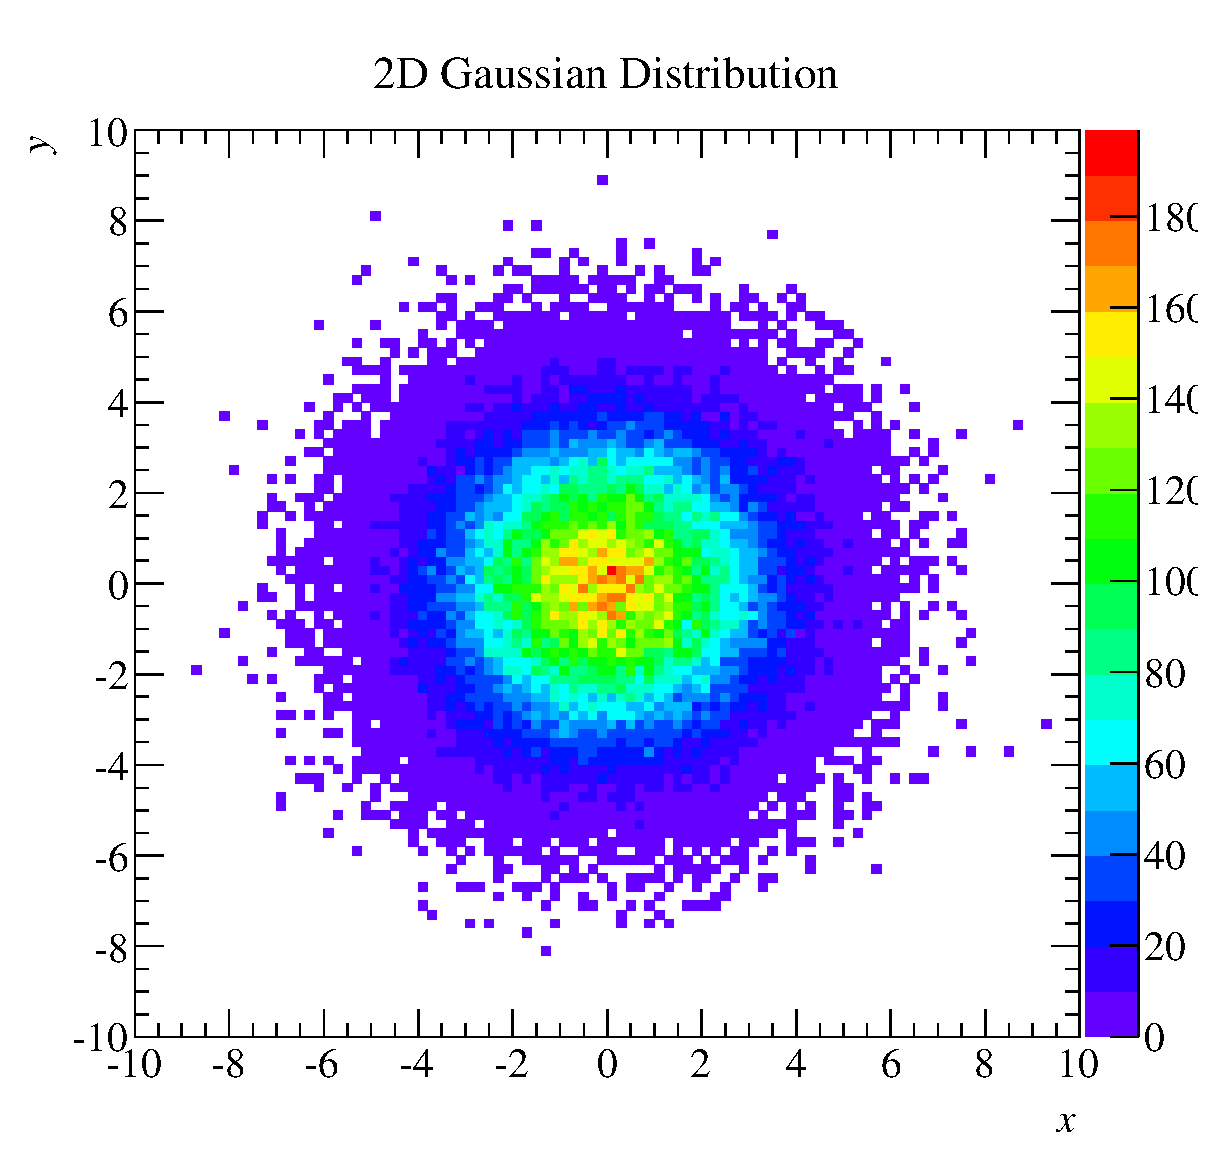
\includegraphics[width=12cm,clip]{fig/TH2D.eps}
  \caption{物理量$x$、$y$(平均$\mu_x = \mu_y = 0$、標準偏差$\sigma = 2$)の 2 次元ガウス分布の例}
  \label{fig_TH2D_eps}
\end{figure}

\section{3次元ヒストグラム}
